\documentclass[11pt]{article}
\usepackage{geometry}                
\geometry{letterpaper}                   

\usepackage{graphicx}
\usepackage{amssymb}
\usepackage{epstopdf}
\usepackage{natbib}
\usepackage{amssymb, amsmath}
\usepackage{color}
\usepackage{listings}
\lstloadlanguages{Matlab} 

\lstset{ %
  language=Matlab,						% choose the language of the code
  basicstyle=\scriptsize,		% the size of the fonts that are used for the code
  numbers=left, 							% where to put the line-numbers
  numberstyle=\tiny,	% the size of the fonts that are used for the line-numbers
  stepnumber=1,								% the step between two line-numbers. If it's 1 each line will be numbered
  numbersep=5pt,							% how far the line-numbers are from the code
  backgroundcolor=\color{white},	% choose the background color. You must add \usepackage{color}
  showspaces=false, 					% show spaces adding particular underscores
  showstringspaces=false,			% underline spaces within strings
  showtabs=false,							% show tabs within strings adding particular underscores
%	rulecolor=\color{black},    % if not set, the frame-color may be changed on line-breaks within not-black text (e.g. commens (green here)
  frame=single,								% adds a frame around the code
  tabsize=2,									% sets default tabsize to 2 spaces
  breaklines=true,						% sets automatic line breaking
  breakatwhitespace=false,		% sets if automatic breaks should only happen at whitespace
	title=\lstname,             % show the filename of files included with \lstinputlisting;
                              % also try caption instead of title
  escapeinside={\%*}{*)}, % if you want to add a comment within your code
  morekeywords={*,...}, % if you want to add more keywords to the set
  keywordstyle=\color[rgb]{0,0,1},
  commentstyle=\color[rgb]{0.133,0.545,0.133},
  stringstyle=\color[rgb]{0.627,0.126,0.941},
}

\usepackage[bookmarks=true,backref=page]{hyperref}
\hypersetup{%
%		bookmarks=true,         % show bookmarks bar?
    unicode=true,          % non-Latin characters in Acrobat’s bookmarks
    pdftoolbar=true,        % show Acrobat’s toolbar?
    pdfmenubar=true,        % show Acrobat’s menu?
    pdffitwindow=false,     % window fit to page when opened
    pdfstartview={FitH},    % fits the width of the page to the window
    pdftitle={Intersection Problem},    % title
    pdfauthor={Marcel Arikan, Nuhro Ego, Ralf Kohrt},     % author
    pdfsubject={Modelling and Simulating Social Systems with MATLAB at ETHZ},   % subject of the document
    pdfcreator={MiKTeX, LaTeX with hyperref and KOMA-Script},   % creator of the document
    pdfproducer={MiKTeX, LaTeX with hyperref and KOMA-Script}, % producer of the document
    pdfkeywords={Crossroads vs. Roundabouts, Roundabout, Crossroad, MSSSM, Report, Experiment,
								Matlab, ETH Zurich, ETHZ}, % list of keywords
    pdfnewwindow=true,      % links in new window
		pdfpagemode=UseOutlines,	% Inhaltsverzeichnis anzeigen beim Öffnen
		pdfdisplaydoctitle=true,	% Dokumenttitel statt Dateiname anzeigen.
		pdflang=en,							%	Sprache des Dokuments.
    colorlinks=false,       % false: boxed links; true: colored links
    linkcolor=red,          % color of internal links
    citecolor=green,        % color of links to bibliography
    filecolor=magenta,      % color of file links
    urlcolor=cyan,           % color of external links
%		menucolor=blue,					% Farbe festlegen.
		bookmarksnumbered=true,	% Überschriftsnummerierung im PDF Inhalt anzeigen.
		bookmarksopen=true,			%
		bookmarksopenlevel=1,		%
		breaklinks=true,				%
%		bookmarksdepth = 4, 		% of whatever level you want
}




\DeclareGraphicsRule{.tif}{png}{.png}{`convert #1 `dirname #1`/`basename #1 .tif`.png}

%\title{Intersection Problem}
%\author{Marcel Arikan, Nuhro Ego, Ralf Kohrt}
%\date{date} 

\begin{document}



\include{sections/titlepage}
\include{agreement_for_free_download}
%%%%%%%%%% Table of content %%%%%%%%%%%%%%%%%

\tableofcontents

\newpage

%%%%%%%%%%%%%%%%%%%%%%%%%%%%%%%%%%%%%%%
\section{Abstract}
In our simulation, based on cellular automata, we have tried to compare roundabouts to crossroads, controlled by traffic lights, with respect to the traffic flow. We defined the traffic flow as the product of car density and average speed of the cars. Whereever reasonable, the Nagel-Schreckenberg model has been implemented. The main input parameters are car density and pedestrian density. There are three different signalisation modes of the trafficlight, depending on the pedestrian density. We expected roundabouts to be more efficient at low pedestrian densities for every car-density, but if pedestrian density rises the advantage should melt. Indeed, we have found, that the flow decreases approximately linearly to zero with the pedestrian-density rising after having reached the maximum in roundabouts. In contrast, the flow in crossroad is, as expected, rather low but never vanishes. 
\input{sections/individual_contributions}
\section{Introduction and Motivations}
Several groups in this course have simulated roundabouts and crossroads before. Our work is a development of and in addition to �Traffic Dynamics�, written by Tony Wood and Bastian B�cheler in May 2010. In difference to their simulation we added pedestrians and implemented crossroads with lights instead of �priority to the right� organisation. They showed impressively, that roundabouts are much more efficient than crossroads, nearly independent of the car density. They have concluded, that �their model confirms, that the increase in popularity of roundabouts over the last years is justified�. In our view one important parameter was missing: the pedestrian density. As we have lived so far in cities, we have had occasions enough to observe that in the mornings and evenings some large roundabouts are just blocked, when pedestrians are allowed to cross the streets, especially when in the middle of the roundabout is a station for trams or buses. Depending on the pedestrian density we have implemented three different signalisation modes in the crossroads. For high pedestrian densities there won't be any conflicts between pedestrians and cars. So we thought that at least at this stage, crossroads may be in advantage to roundabouts. 
Some results
\section{Description of the Model and Implementation}

\subsection{Description of the main loop}

In our model one can compare roundabouts with crossroads, controlled by traffic lights (which we will call \texttt{crosslight}), with each other. One can use an arbitrary combination of roundabouts and crosslights in a $N \times M$ map. \\
The simulation can be done with different probabilities for the car to go straight and left and right will have the same probability but depend on the probability ahead. One can also choose different car and pedestrian densities. 
The simulation will generate a plot over these densities as x- and y- axis and the average flow and average speed as z-axis. 

\begin{center} 
$flow = density \cdot speed$
\end{center}

\subsubsection{Implementation}

We have a big matrix which shows all roads and intersections. And many smaller ones, 2 for every lane, which contain all the lanes for every road after each other. 
The first one contains the positions of the cars and the second one contains their speed. And one for every array which is used by a \texttt{crosslight} or roundabout intersection and needs to be stored for calculating the next step.\\

For almost every one of those arrays we have to arrays, one for the current state which is shown on the screen and one for the next step which contains the next step, which will be calculated cell for cell. 
After the calculation the next step will be stored in the first array and the calculation starts over again.

\subsection{Roundabout}
Our implementation of the roundabout consits of a circle with 12 cells and 4 roads, which lead towars it. Every street has pedestrian crossings in front of each roundabout. 
Like in the real world, cars inside the roundabout have priority over cars wanting to enter them and pedestrians have priorithy over cars at the pedestrian crossings, 
with the addition, that pedestrians will only walk on the road if there is no car staying or driving on the cell they wants to walk on. 
Inside the crossroad the speed a car can have is limited to 1 cell per iteration. \\

A car which wants to leave the roundabout at the next exit will indicate, in our plot this is shown by giving these cars a darker colour. 
The exit a car will take is calculated from the probability ahead like in the crossroad, but with a fixed probability of 5 \% for a car which will take the 4th exit (i.e. the car will turn around). \\
\subsubsection{Implementation}
This is implemented with many arrays, three arrays for the circle, one which shows whether there is a car or not and if the car wants to leave at the next exit. 
The second is used to store the velocity of the car and the third is used to store how many exits the car will pass without leaving.\\

For the pedestrians we use a yellow colour on the street (a car is blue), and two 'buckets' between the lanes of each road so that they will cross both lanes of a road.
\section{Simulation Results and Discussion}

{\centering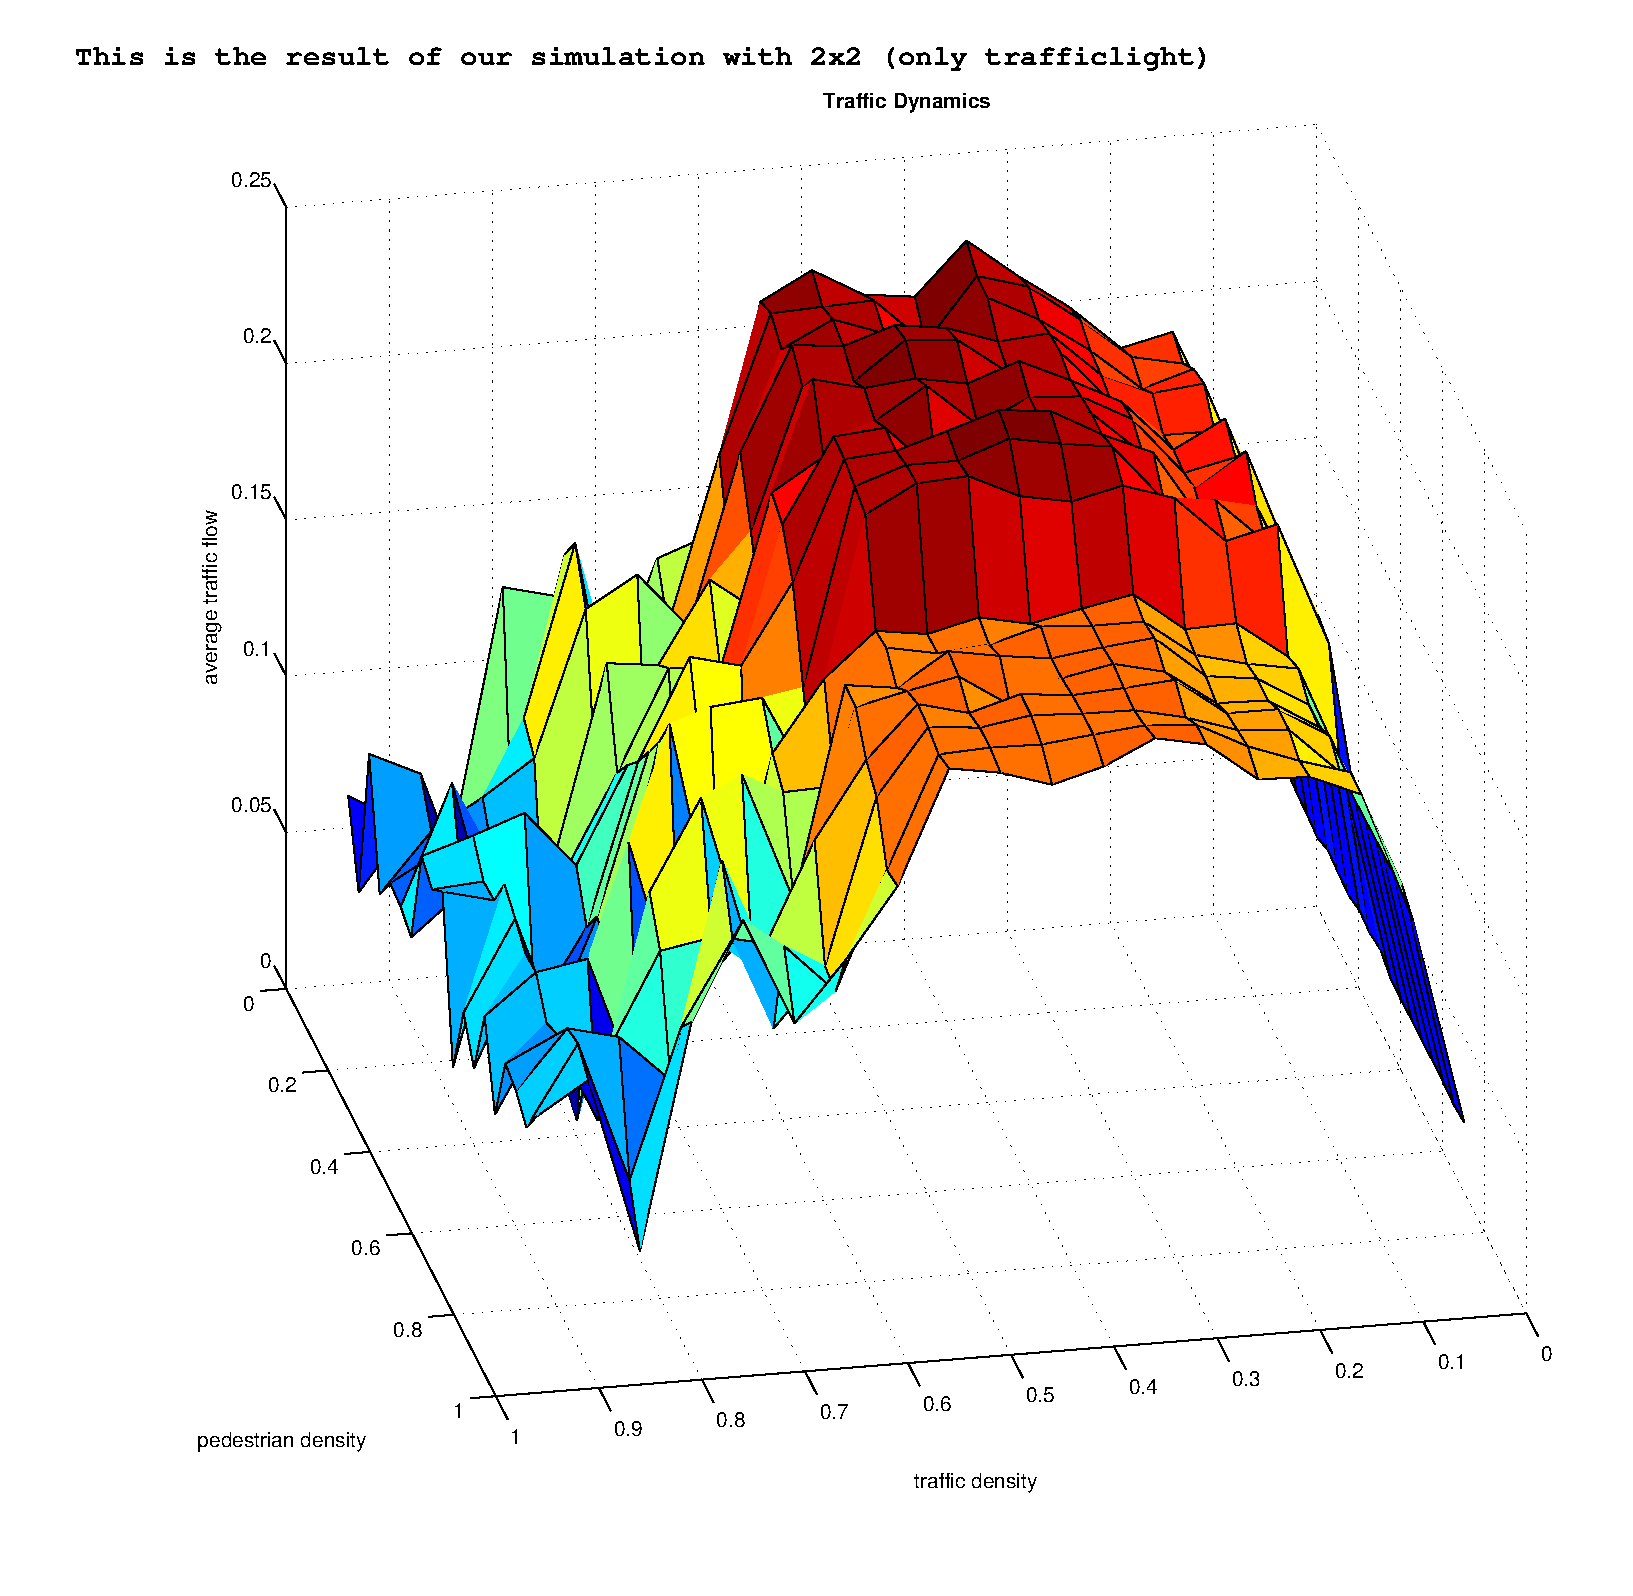
\includegraphics[width=15cm]{images/2-2-trafficlight.eps}


{\centering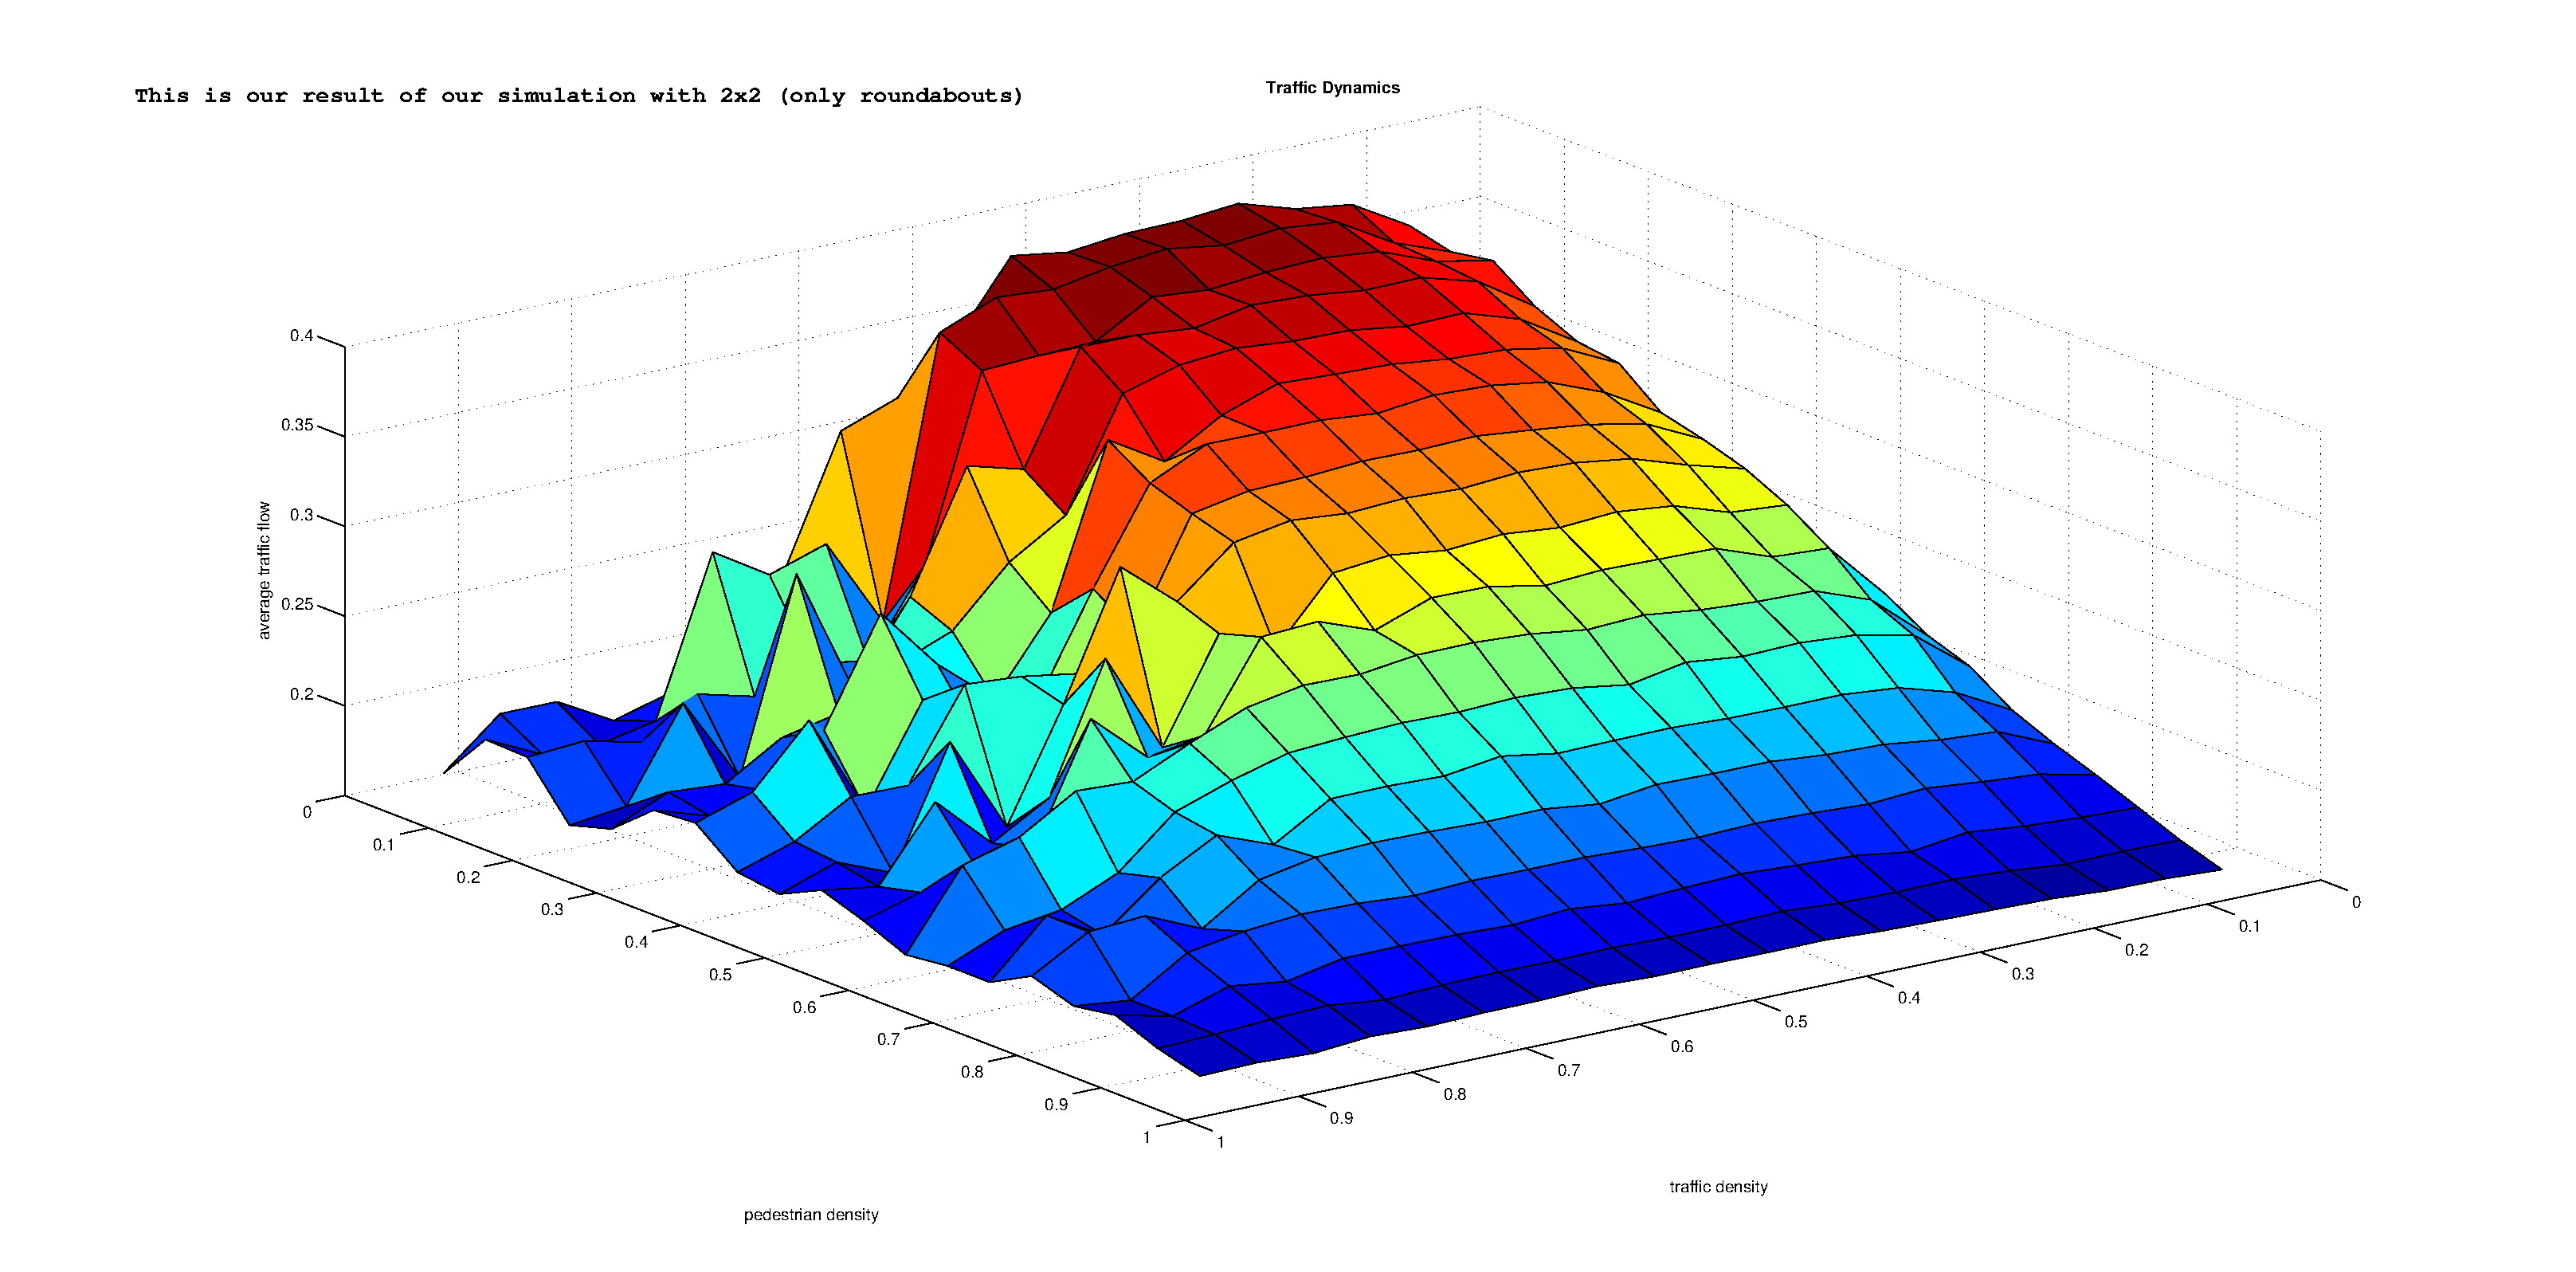
\includegraphics[width=15cm]{images/2-2-roundabout.eps}

{\centering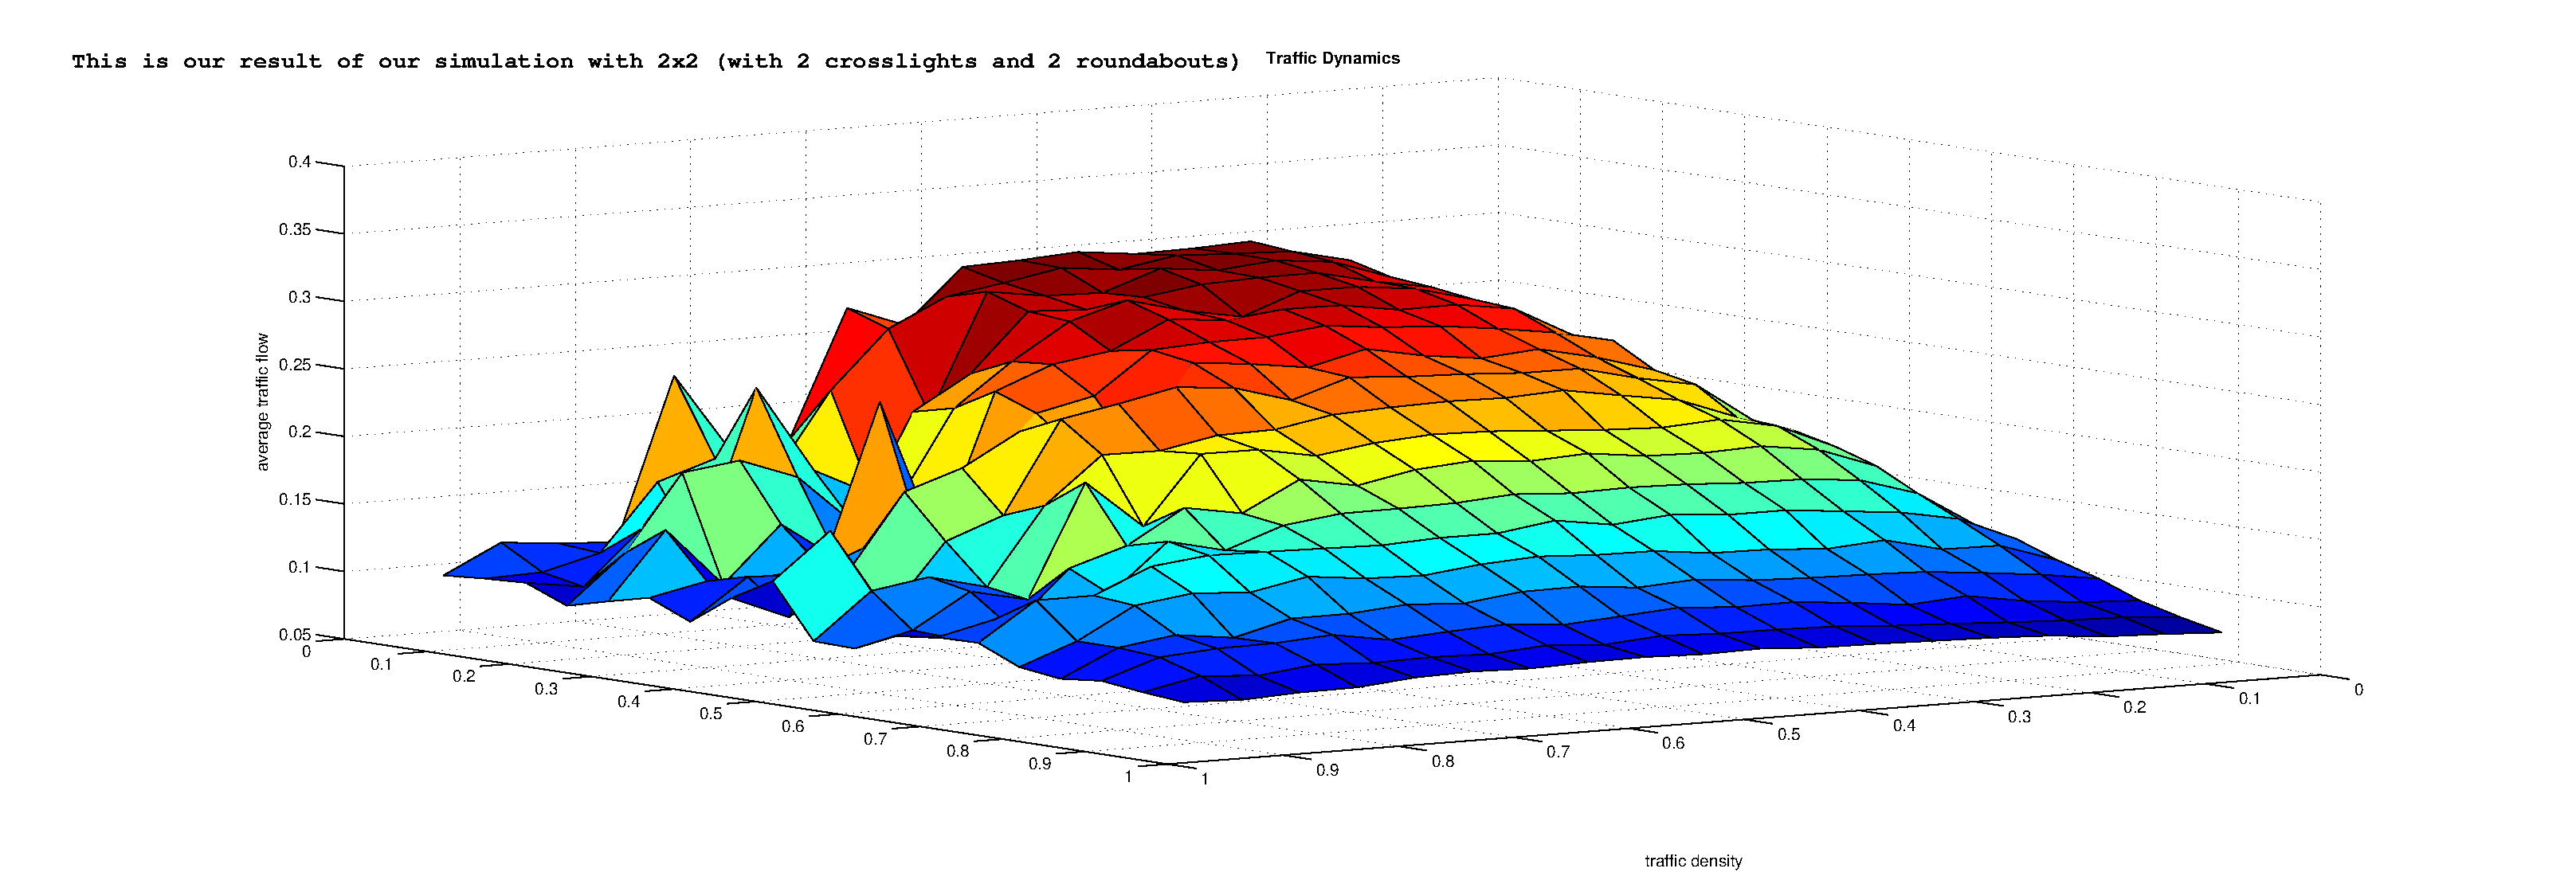
\includegraphics[width=15cm]{images/2-2-mix.eps}

{\centering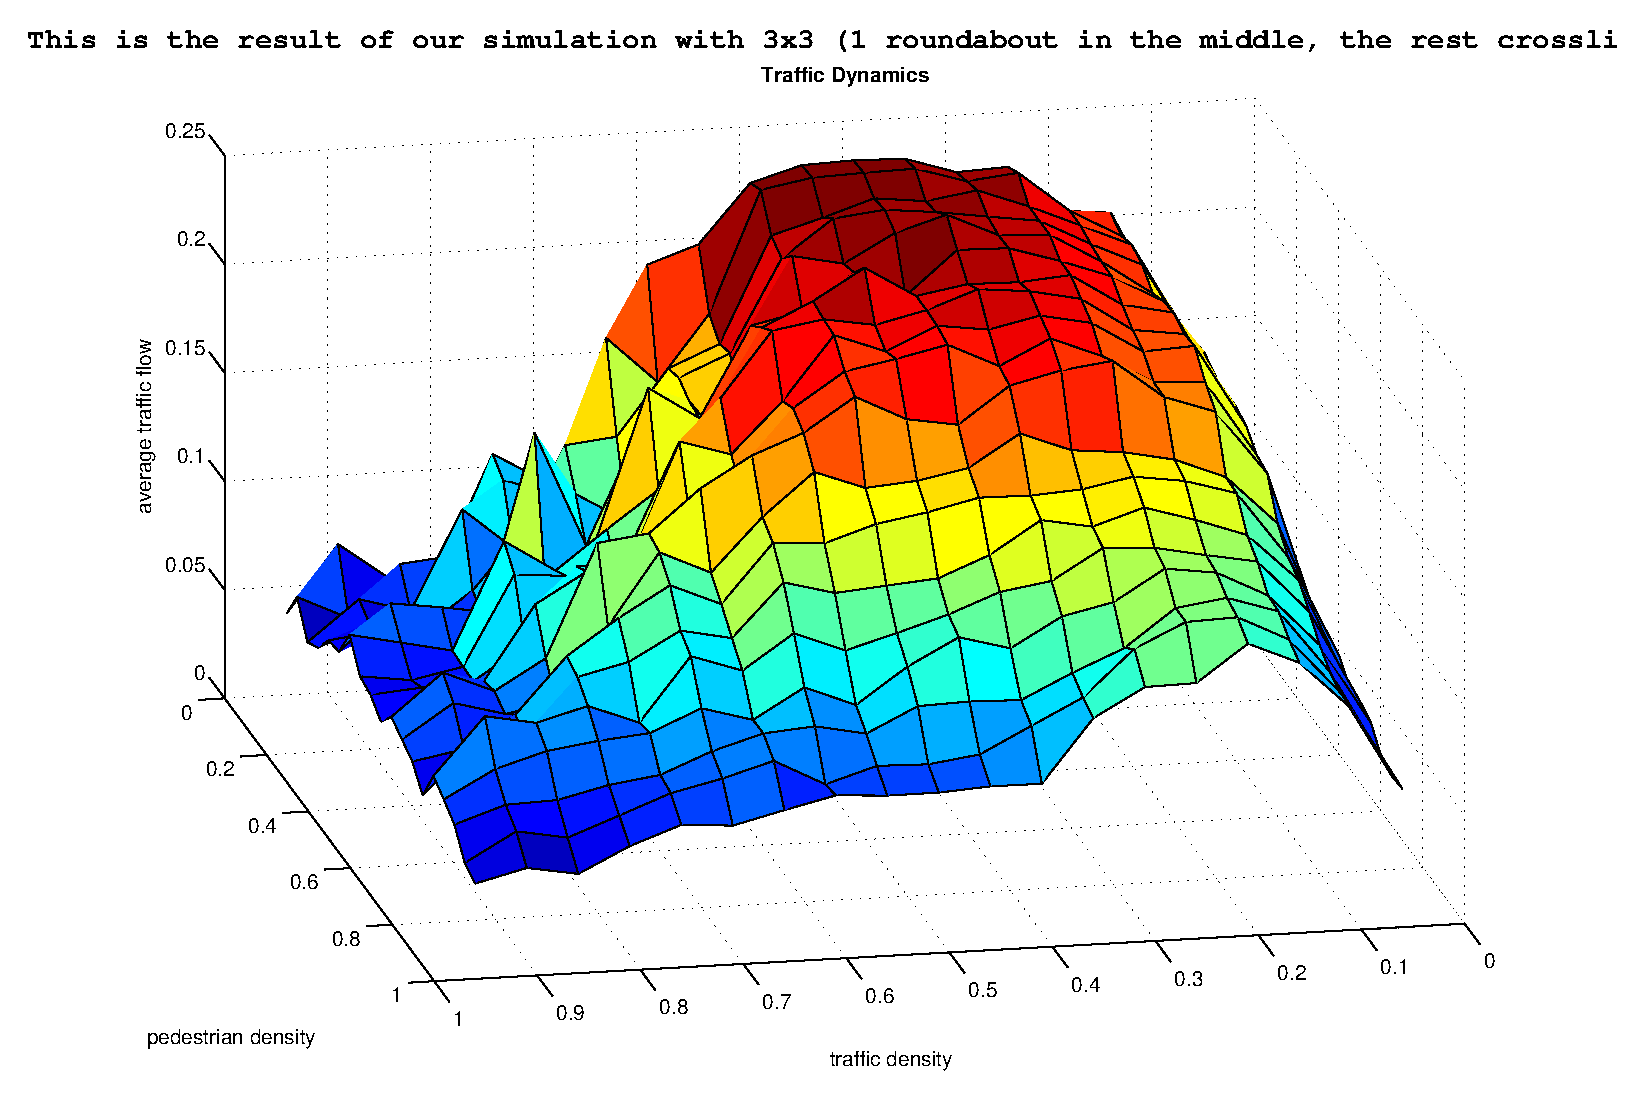
\includegraphics[width=15cm]{images/3-3-mix.eps}

{\centering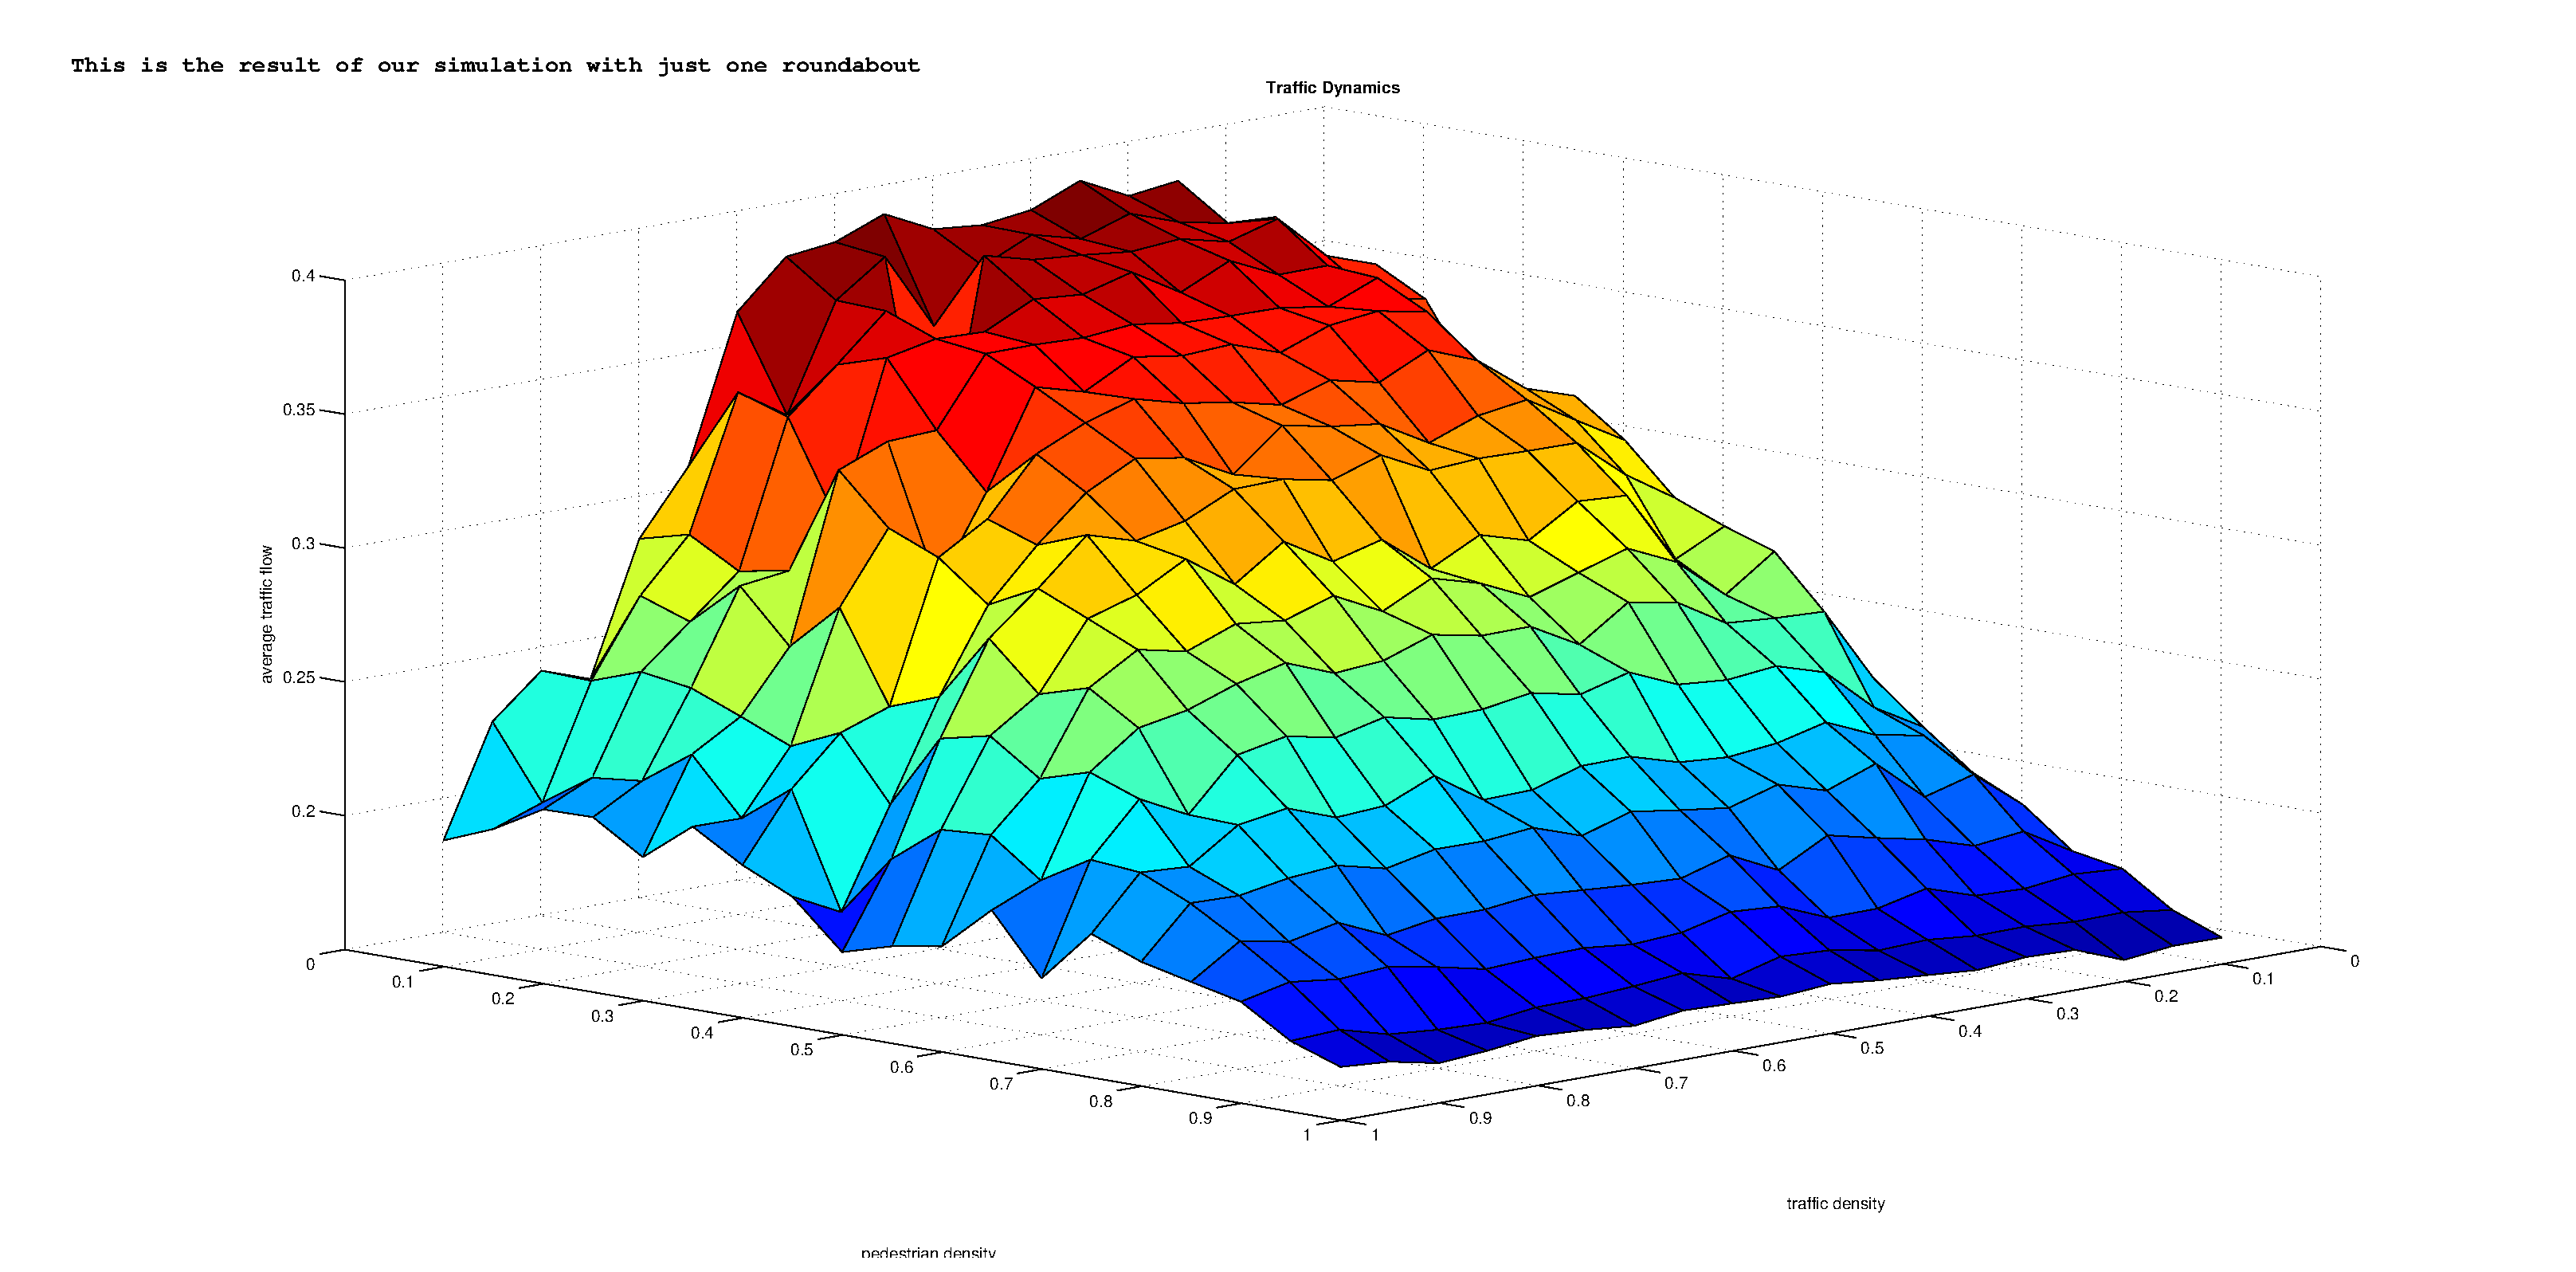
\includegraphics[width=15cm]{images/1-1-roundabout.eps}

{\centering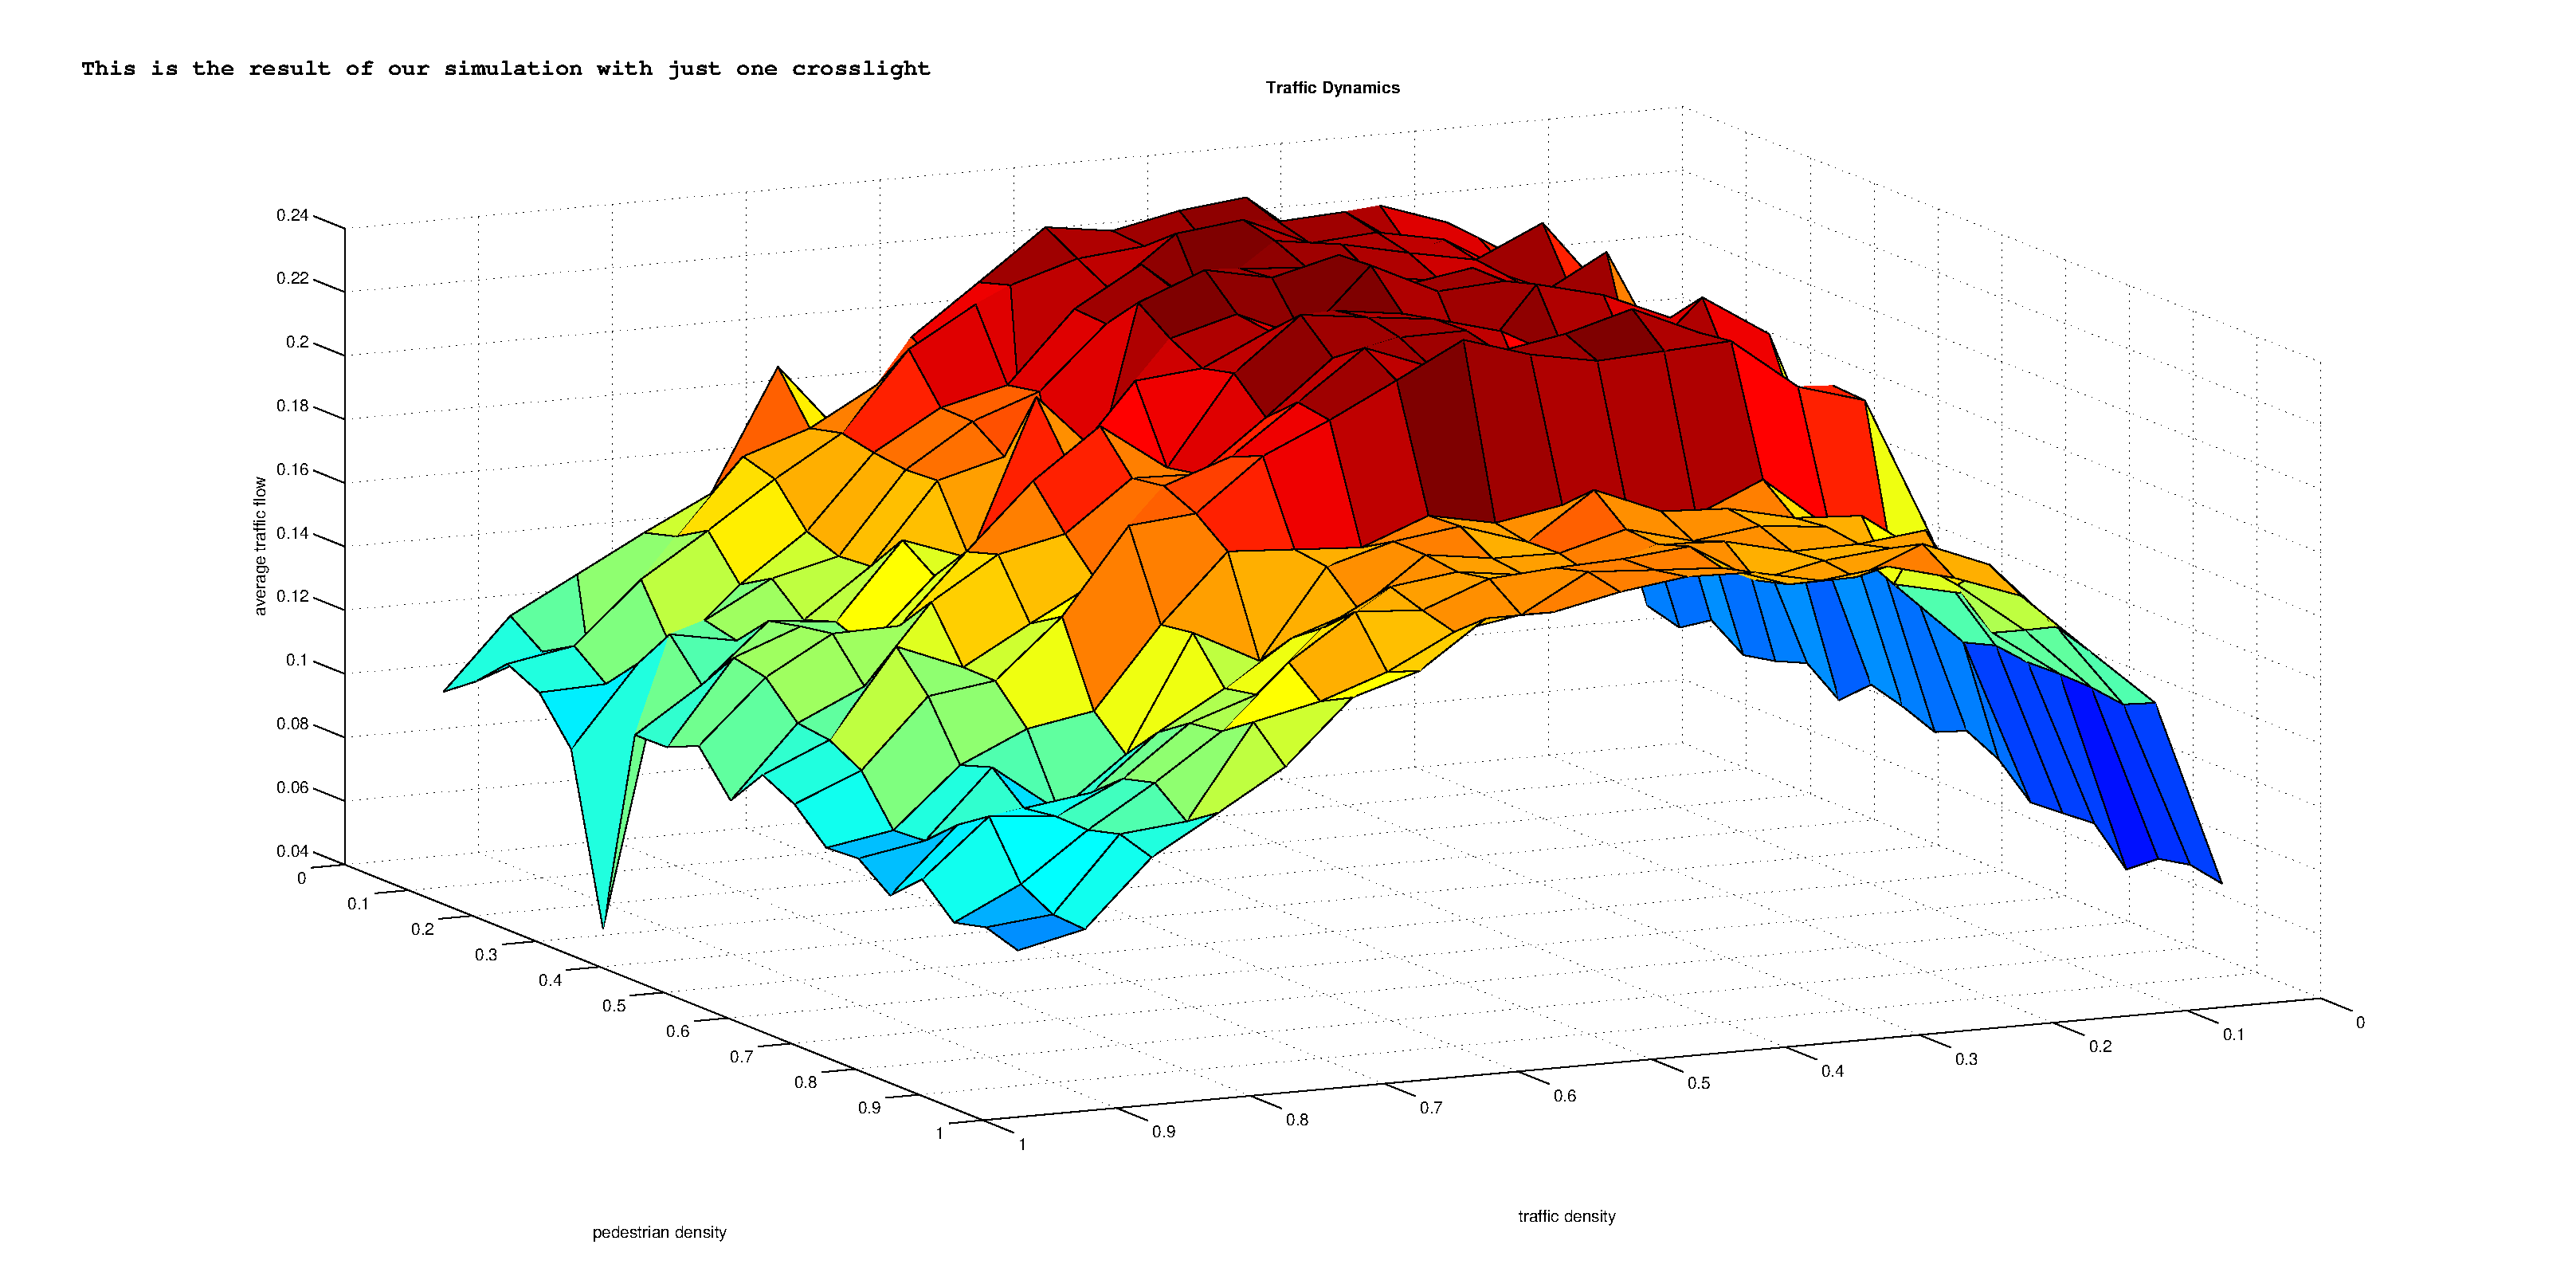
\includegraphics[width=15cm]{images/1-1-trafficlight.eps}
\section{Summary and Outlook}
The results reflect our expectation very well. At low pedestrian densities the simulation is comparable to the one of Wood and B�cheler with no pedestrians at all. As expected, roundabouts are much more sensitive to pedestrians than crossroads. Crossroads keep their functionality to very high pedestrian densities, whereas roundabouts collapse. So it's quite reasonable to use crossroads in cities. But the maximum traffic flow in roundabouts can be twice as high than in cross rounds. For highways outside cities, roundabouts can therefore be a good choice, especially because they are simple and they normally need more space than crossroads. So, as always in life, every system as its advantages under certain conditions. 


There are many possible modifications to develop in this simulation. As mentioned in the description, an intelligent control of the traffic light could may boost the efficiency of crossroads. Vice versa a traffic light at the entry of a roundabout kicked in at high pedestrian densities could improve the efficiency and avoid a collapse. It would be interesting to analyse and simulate different hybrid models, for example with a mixed city configuration of crossroads and roundabouts, or using these controlled roundabouts.  

\appendix
\listoffigures

\clearpage
\section{Listings}
\label{sec:Listings}

\subsection{Matlab Codes}


\lstinputlisting[language=Matlab,caption={traffic.m},label=traffic]{../../code/traffic.m}
\lstinputlisting[language=Matlab,caption={trafficloop.m},label=trafficloop]{../../code/trafficloop.m}
\lstinputlisting[language=Matlab,caption={trafficsim.m},label=trafficsim]{../../code/trafficsim.m}
\lstinputlisting[language=Matlab,caption={measure-gap.m},label=measure_gap]{../../code/measure_gap.m}
\lstinputlisting[language=Matlab,caption={connection.m},label=connection]{../../code/connection.m}
\lstinputlisting[language=Matlab,caption={pdestination.m},label=pdestination]{../../code/pdestination.m}
\lstinputlisting[language=Matlab,caption={schreckenberg.m},label=schreckenberg]{../../code/schreckenberg.m}
\lstinputlisting[language=Matlab,caption={roundabout.m},label=roundabout]{../../code/roundabout.m}
\lstinputlisting[language=Matlab,caption={crosslight.m},label=crosslight]{../../code/crosslight.m}
\lstinputlisting[language=Matlab,caption={crosslight-measure-gap.m},label=crosslight_measure_gap]{../../code/crosslight_measure_gap.m}
\lstinputlisting[language=Matlab,caption={crosslight-next-ij.m},label=crosslight_next_ij]{../../code/crosslight_next_ij.m}
\lstinputlisting[language=Matlab,caption={plotresults.m},label=plotresults]{../../code/plotresults.m}
\lstinputlisting[language=Matlab,caption={plot-map.m},label=plot_map]{../../code/plot_map.m}

\clearpage
\bibliographystyle{plain}
\bibliography{bib/references}


\end{document}  



 
